\documentclass{../template/labo}

\usepackage[utf8x]{inputenc}
\usepackage[T1]{fontenc}
\usepackage{ucs}
\usepackage{amsthm} %numéroter les questions
\usepackage{amsmath}
\usepackage[frenchb]{babel}
\usepackage{datetime}
\usepackage{xspace} % typographie IN
\usepackage{hyperref}% hyperliens
\usepackage[all]{hypcap} %lien pointe en haut des figures
\usepackage[french]{varioref} %voir x p y
\usepackage{fancyhdr}% en têtes
\usepackage[]{graphicx} %include pictures
\usepackage{tikz}
\usetikzlibrary{babel,positioning,calc}
\usepackage[siunitx]{circuitikz}
\usepackage{mathastext} % math as standfard text : units are respecting typography conventions.
\usepackage{siunitx}
\usepackage{amssymb}
\usepackage{gnuplottex}
\usepackage{ifthen}
\usepackage{xcolor}
\usepackage{float}
%\usepackage{footmisc}
\usepackage[normalem]{ulem}

%\usepackage[top=1.3 in, bottom=1.3 in, left=1.3 in, right=1.3 in]{geometry} % Yeah, that's bad to play with margins
\usepackage[]{pdfpages}

\usepackage[]{attachfile}

%%%%%%%%%%%%
% Tables
%%%%%%%%%%%%
\usepackage{booktabs}
\renewcommand{\arraystretch}{1.1} % Opens up the table a tad
\usepackage{multicol}
\usepackage{multirow}

\langexam{frenchb}

\newboolean{koriG}
\ifx\koriG\undefined
\correction{false}
\else
\correction{true}
\fi

% \correction{false}
%\correction{true}

\author{The Fantastic Four} %<3

\pagestyle{fancy}
\lhead{[ELEC-H-301] Électronique appliquée\\ LABO \no 3 : Transistor MOS\ifthenelse{\boolean{corrige}}{~-- corrigé}{}}
\rhead{v2.1.1\\ page \thepage}
\cfoot{}
%%

\pdfinfo{
/Author (ULB -- BEAMS)
/Title (LABO 3 ELEC-H-301, Transistor MOS)
/ModDate (D:\pdfdate)
}

\hypersetup{
pdftitle={LABO 3 [ELEC-H-301] Électronique appliquée: Transistor MOS},
pdfauthor={ULB - BEAMS},
pdfsubject={Filtrage}
}


\setlength{\parindent}{0pt}

\begin{document}

\tptitle{}{Séance 3~: Réalisation d'un ampli à transistor}



% ########   ##      ##  ##########  ########     #####    
%    ##      ###     ##      ##      ##     ##  ##     ##  
%    ##      ## ##   ##      ##      ##     ##  ##     ##  
%    ##      ##  ##  ##      ##      ########   ##     ##  
%    ##      ##   ## ##      ##      ##   ##    ##     ##  
%    ##      ##     ###      ##      ##    ##   ##     ##  
% ########   ##      ##      ##      ##     ##    #####    

\section{Introduction}

Les passages nécessitant des pré-déterminations ou des réflexions théoriques sont indiqués par un symbole \faCogs~ dans la marge,
ceux nécessitant de manipuler du matériel par le symbole \faFlask~ et les passages informatif par \faLightbulbO.

\subsection{But de la manipulation et objectifs d'apprentissage}

Le but de ce laboratoire est de réaliser un pré-amplificateur audio pour une radio AM en utilisant un transistor MOS.
Ce pré-amplificateur est un amplificateur de classe A, particulièrement apprécié des audiophiles mais ayant un mauvais rendement.\\


À la fin de ce laboratoire, vous devez être capable :
\begin{itemize}
\item de réaliser le pré-amplificateur audio avec un étage source commune
\item d'expliquer le fonctionnement de l'étage source commune et sa polarisation.
\item d'utiliser le mode XY d'un oscilloscope.
\end{itemize}

\subsection{Prérequis}
\begin{itemize}
\item Chapitre \no 17 du livre de référence (ed 5)
\item Circuit RC du premier ordre.
\item TP \no 2, exercice 6 sur la polarisation
\item TP \no 5 portant sur les transistors MOS

\end{itemize}

\subsection{Matériel}

\begin{center}
	\begin{tabular}{p{0.2\textwidth}rlp{0.1\textwidth}}
		Composant & \multicolumn{2}{c}{Valeur} & Quantité \\\toprule
		\multirow{5}{*}{Résistance} & 56 & $\si{\ohm}$ & x1 \\
									& 100 & $\si{\ohm}$ & x1 \\
									& 150 & $\si{\ohm}$ & x1 \\
									& 10 & $\si{\kohm}$ & x2 \\
									& 30 & $\si{\kohm}$ & x1 \\\midrule
		\multirow{1}{*}{Condensateur} 	& 10 & $\si{\nano\farad}$ & x2 \\\midrule
		Transistor TN0604N3-G & & & x1 \\\bottomrule
	\end{tabular}
	\end{center}

\subsection{Prédéterminations}

Les déterminations des questions \ref{Q:det_rd}, \ref{Q:vout_th} et \ref{Q:capa_inout} doivent être faites avant l'arrivée au laboratoire.
Le TP 5 portant sur les transistors MOS fait également office de prédéterminations.


% ########   ##     ##  
%    ##      ##     ##  
%    ##      ##     ##  
%    ##      ##     ##  
%    ##       ##   ##   
%    ##        ## ##    
% ########      ###   
\section{Caractérisation du transistor}

\begin{info}
Le transistor utilisé dans ce laboratoire est un TN0604N3-G. Référez-vous à sa fiche technique lorsque des résultats analytiques sont demandés.

Avant de dimensionner l'étage en source commune, il est nécessaire de caractériser le transistor afin de déterminer sa transconductance $g_m$. % pour un point de fonctionnement donné.
On cherche en particulier à déterminer sous quelles conditions il se comporte comme une source de courant commandée en tension.
\end{info}

\subsection{Caractéristique $I_D=f(V_{GS})$}

Pour relever la caractéristique $I_D=f(V_{GS})$, vous utiliserez le montage suivant. La résistance $R_D$ sert à limiter le courant traversant le transistor pour ne pas le détruire.
\ctikzset{tripoles/mos style/arrows}
%\begin{figure}[H]
	\begin{center}
		\begin{circuitikz}[scale=0.8]%[american voltages]
		\draw
		(0,0) to [V=$e(t)$] (0,2)
		(0,2) to [short] (1,2)
		(0,0) to (1,0)
		(1,2) to [open, v^<=$V_{GS}$](1,0)
		(1,0) to [short, o-] (2,0)
		(3,2) node[nfet] (mos) {}
		(3,0) to [short] (mos.S)
		(1,2) to [short] (mos.G)
		(mos.B) -- (mos.S)
		(2,0) to (3,0)
		(mos.D) to [short, i<=$I_D$](3,3)
		(3,3) to [R,l=$R_D$ ] (3,5)
		%(3,3.2) to [short] (4,3.2)
		(3,5) to (4,5)
        %(4,3.2) node[esource] (voltm) {V}
		%(4,3.2) to (4,5)
		%(2,0) -- (5,0) to [battery, l_=$12V$] (5,5) -- (3,5)
		(2,0) -- (5,0)
		(5,5) -- (3,5)
		(5,5) to [battery, l=$5V$] (5,0)
		(3,0) node[ground] {}
		;\end{circuitikz}
	\end{center}
	\vspace*{-0.5cm}
%\caption{Montage pour relever $I_D=f(V_{GS})$}
%\label{fig:scidvgs}
%\end{figure}

\begin{predet}
\Question{\label{Q:det_rd}
Déterminez $R_D$ tel que le transistor ne dissipe pas plus de $65 \si{\milli\watt}$. 

\begin{astuce}
	Trouvez d'abord l'expression de la puissance dissipée par le transistor en fonction de son courant de drain $I_D$. Trouvez ensuite la valeur de $I_D$ maximisant la puissance.
\end{astuce}
}
{

$P_T$ est la puissance dissipée par le \textbf{transistor} et $E$ la tension d'alimentation connectée à $R_D$.

$$P_T=V_{DS}\cdot I_D = \left(E-R_D\cdot I_D \right)\cdot I_D$$
d'où : $$ P_T=E\cdot I_D - R_D \cdot {I_D}^2$$

L'extremum (ici : maximum) se trouve en :

$$\frac{\partial P_T}{\partial I_D}=0 \Longleftrightarrow E-2R_D \cdot {I_D}_{max} = 0$$

$$\Longrightarrow {I_D}_{max}=\frac{E}{2R_D}$$

d'où : $${P_T}_{max}=\frac{E^2}{4\cdot R_D}$$

finalement : $$R_D=\frac{E^2}{4\cdot {P_T}_{max}}$$

On obtient finalement : $$R_D=96 \Omega @E=5 V$$

\label{Q:predet}
}
\end{predet}

\begin{manip}

Assemblez ce montage en utilisant un transistor TN0604N3-G et une résistance $R_D$ de 100 $\si{\ohm}$.
\begin{astuce}
	Référez-vous à la documentation technique pour connaître la configuration des pattes du transistor. Faites attention à bien identifier la partie \textit{bombée} du composant et ne mélangez pas les pattes !
\end{astuce}

\Question{
Relevez manuellement des points de la caractéristique  $I_D=f(V_{GS})$ pour $V_{GS}$ compris entre $0V$ et $2V$.

\begin{astuce}
	Pour aller plus loin, vous pouvez directement afficher la caractéristique en utilisant le mode XY de l'oscilloscope. Vous pourrez ainsi observer $V_{DS}$ en fonction de $V_{GS}$. Puisque $I_D = \frac{E-V_{DS}}{R_D}$, on peut retrouver la caractéristique par opération graphique.
\end{astuce}
}
{
}
\end{manip}

\begin{predet}
\Question{
Cette caractéristique est-elle linéaire ou quadratique ?
Peut-on utiliser ce montage pour amplifier des signaux ($V_{in}$)
\begin{itemize}
	\item[$\square$] de grande amplitude ;
	\item[$\square$] de petite amplitude ;
	\item[$\square$] de n'importe quelle amplitude.
\end{itemize}
}
{
La caractéristique n'est pas linéaire. Étant donné qu'il faut une relation linéaire pour obtenir une amplification sans déformation, ce montage ne peut servir d'amplificateur que pour de petits signaux en entrée. À cette faible amplitude, on pourra approximer la relation comme étant linéaire.
}
\end{predet}

\begin{predet}
\Question{
	Quelle est la tension de seuil $V_{th}$ que vous observez ?
	Vérifiez que cette valeur est cohérente avec l'intervalle de valeurs donné dans la fiche technique.
}
{
	La fiche technique indique une tension de seuil (Gate threshold voltage) comprise entre 0.6 et 1.65 $\si{\volt}$.
}
\end{predet}

\begin{predet}
\Question{
Choisissez judicieusement un point de fonctionnement sur le relevé précédent.\\
Munissez-vous ensuite des caractéristiques de sortie du transistor se trouvant en annexe de cet énoncé et tracez-y la droite de charge du transistor pour une tension d'alimentation de $5 \si{\volt}$ et $R_D = 100 \si{\ohm}$.
Indiquez dans quelle zone fonctionne le transistor sur cette droite de charge.

Déduisez-en l'amplitude maximale possible en sortie pour le point de fonctionnement choisi.
\label{Q:Q9}
}{
	Un point de fonctionnement judicieux se trouvera dans la zone « passante » du transistor, c'est-à-dire sur la caractéristique de transfert dans l'abscisse est une tension supérieure à la tension de seuil.
}
\end{predet}
\clearpage


%  #######   ########    #######            #######     #####    ##       ##  
% ##     ##  ##     ##  ##     ##          ##     ##  ##     ##  ###     ###  
% ##         ##     ##  ##                 ##         ##     ##  ## ## ## ##  
%  #######   ########   ##           ####  ##         ##     ##  ##  ###  ##  
%        ##  ##   ##    ##                 ##         ##     ##  ##       ##  
% ##     ##  ##    ##   ##     ##          ##     ##  ##     ##  ##       ##  
%  #######   ##     ##   #######            #######     #####    ##       ##  
\section{Amplifier avec un montage en source commune}

\begin{info}
La partie précédente permet de conclure que l'amplification est possible avec un transistor MOS. Nous allons donc construire un montage amplificateur autour du transistor.


\begin{figure}[H]
%\vspace{-0.3cm}%dirty hack
	\begin{center}
		\begin{circuitikz}[scale=0.8]
		\draw
		(0,0) to [sV=$e(t)$] (0,2)
		(0,2) to [short] (1,2)
		(0,0) to (1,0)
		(1,2) to [open, v^<=$v_{in}$](1,0)
		(1,0) to [short, o-] (2,0)
		(3,2) node[nfet] (mos) {}
		(mos.S) to [short] (3,0)
		(mos.B) -- (mos.S)
		(1,2) to [short] (mos.G)
		(2,0) to (3,0)
		(mos.D) to [short](3,3) %, i<=$I_D$
		(3,3) to [R, l=$\SI{100}{\ohm}$] (3,5)
		(3,3) to [short, -o](4,3)
		(4,3) node[anchor=west] {$v_{out}$}
		(3,5) node[rground, yscale=-1] (alim) {}
		(3,5.7) node {+5V}
		(3,0) node[ground] {}
		;\end{circuitikz}
	\end{center}
%\vspace{-0.7cm}%dirty hack
\caption{Montage à améliorer}
\label{fig:scidt}
\end{figure}
\end{info}

\begin{predet}
\Question{\label{Q:vout_th} Déterminez théoriquement la \textbf{forme} du signal de sortie $v_{out}$ pour $$v_{in}=V_{max}\cdot \sin (2\pi \cdot f \cdot t)$$ avec $V_{max}=2V$, $V_{TH}\simeq 0.6V$ et $f=10 kHz$.
}{}
\end{predet}

\begin{manip}
\Question{Vérifiez expérimentalement la forme de $V_{out}$.

Donndez \textbf{deux raisons} pour lesquelles ce circuit ne convient pas pour réaliser un amplificateur linéaire ?
Comment pourriez-vous régler ces problèmes ?
\label{Q:2elts1}
}
{
\begin{enumerate}
	\item Le signal de sortie est écrêté et non linéaire.
	\item Sa moyenne est non nulle. C'est un problème dans le cadre d'una application audio, un signal de sortie à moyenne non-nulle allant polariser le haut-parleur, l'abîmant ou dégradant la qualité audio.
	\item L'amplification est non-linéraire.
\end{enumerate}

Comment les régler : 
\begin{enumerate}
    \item Ajouter une composante continue pour se placer dans la zone de saturation $\Longrightarrow$ ajout d'une tension de polarisation.
    \item Ajouter un filtre passe haut en sortie pour filtrer la composante continue.
    \item Diminuer l'amplitude du signal d'entrée.
\end{enumerate}
\label{Q:2elts2}
}
\end{manip}

\begin{manip}
\Question{~
    Manipulez votre signal $V_{in}$ pour essayer d'améliorer la forme de $V_{out}$.
\begin{astuce}
	Le générateur possède une fonctionnalité « \textit{offset} » permettant de décaler le signal positivement ou négativement.
\end{astuce}
}
{}
\end{manip}

\begin{predet}
\Question{~
\begin{itemize}
    \item \label{Q:capa_inout} Comment injecter un signal à moyenne nulle dans ce circuit en considérant les corrections apportées au circuit à la question précédente ?
    \item De même, que faire pour obtenir une tension de sortie à moyenne nulle ?
\end{itemize}
}
{
On ajoute une capacité de découplage en entrée et en sortie et un pont résistif pour la polarisation.
}
\end{predet}


\begin{info}
	Vous devriez obtenir le montage suivant :
	\begin{center}
		\begin{circuitikz}[scale=1]\draw
			(0,1) to [short,o-] (9,1)
			(4,6) to [short] (9,6)
			(0,3) node[anchor=east] {In} to [short,o-] (1,3)
			(0,3) node[anchor=south]{} to [open, v_<=$V_{in}$]  (0,1) 
			(1,3) to [C=$C_{in}$ ](1.5,3) 
			(1.5,3) to [short,-*] (2,3) node[anchor=south west]{}
		
			(2,6) node[anchor=south ] (alim) {$+V_{DC}$}
			(1.6,6) -- (2.4,6) %bar under the label
			(2,3) to [R, l_=$R_{B1}$](2,6)
			(2,3) to [R=$R_{B2}$](2,1)
			(4,3) node[nfet] (mos) {}
			(mos.G) to [short] (2,3)
			(mos.D) to (4,4) to [R, l_=$R_D$] (4, 6)		
			(mos.D) to [short,-*](4,3.5)  to [short] (4.25,3.5)
			(mos.S) to [short] (4,1)% to [short, -o](2,0)  node[anchor=west] {S}
			(mos.S) -- (mos.B) %source to bulk connection		
		
			(4.25,3.5) node[anchor=south]{} to [C, l^=$C{out}$] (6,3.5) to  [short](6,3.5)node[anchor=south]{} to [short,-o](6.5,3.5)node [anchor=south] {Out}	
			(6,3.5) to [generic, l_=$R_{ch}$] (6,1)
			(6.5,3.5) to [open,v^<=$V_{out}$] (6.5,1)
			(9,6) to [battery, l_=$E$](9,1)
			(4,1) node[circ]{}
			(4,1) node[ground]{}
			;\end{circuitikz}
	\end{center}
\end{info}

\begin{manip}
\Question{Réalisez ce montage avec $V_{DC} = 5 V$, $E = 5 V$, $C_{in} = C_{out} = 10 \si{\nano\farad}$ et $R_{B1} = 30 \si{\kohm},\ R_{B2} = 10 \si{\kohm}$.
Dans un premier temps, considérez un montage à vide, c'est-à-dire sans résistance de charge $R_{ch}$.}{}
\end{manip}

% \begin{info}
% Les réponses aux questions \ref{Q:gain} à \ref{Q:pchg} doivent être étayées par des vérifications expérimentales.
% \end{info}

\begin{predet}
\Question{Exprimez $V_{out}$ en fonction de $V_{in}$ et des différents paramètres de votre montage.
Quel est le gain de votre montage ?
\begin{astuce}
	Utilisez une représentation du montage à petit signal.
\end{astuce}
\label{Q:gain}
}
{
$$V_{out} = V_{ds}=-g_m\cdot R_D \cdot V_{in}$$

Bien que cette relation soit valable quel que soit le régime de fonctionnement du transistor, seule la partie où le $g_m\neq 0$ est intéressante pour l'application.
}
\end{predet}

\begin{manip}
\Question{ Vérifiez expérimentalement votre résultat.
	\begin{astuce}
	Le mode XY de l'oscilloscope vous permet d'afficher directement $V_{out}$ (i.e. $V_{ds}$) en fonction de $V_{in}$ (i.e. $V_{gs}$).
	Chargez votre montage avec $R_{ch} = 10 k\Omega$ pour réduire le déphasage entre les signaux.
	\end{astuce}
	Indiquez sur votre relevé les limites d'écrêtage et de linéarité, comparez avec le résultat de la question~\ref{Q:Q9}.
}
{
Utilisation du mode XY :
mettre un signal triangulaire ($10kHz$, quelques volts) à l'entrée du montage, afficher $V_{out}=f(V_{in})$ sur l'oscillo.

 Il peut être nécessaire de charger un peu la sortie avec une résistance, en particulier pour diminuer la fréquence de coupure du filtre passe-haut en sortie.
 Étant donné que cette charge est bien plus élevée que l'impédance de sortie de l'étage amplificateur, elle aura un impact limité sur le gain de ce dernier (on obtient $A = -g_m \cdot (R_D // R_{ch})$).

Le mode XY permet de constater l'effet de la polarisation sur le gain et sur l'écrêtage du signal.
}
\end{manip}

% \Question{~
% \label{Q:PF}
% \begin{itemize}
%     \item Quelle est l'influence de la composante continue sur les caractéristiques du montage ?
%     \item Quelle est la valeur de la composante continue qui maximise l'excursion en sortie ? Qui maximise le gain ? Avec quel inconvénient ?
% \end{itemize}
% }
% {
% Utiliser le potentiomètre pour modifier a polarisation. On constate le changement de gain sur le tracé XY précédent.

% La polarisation est idéale si le point $(0,0)$ fait partie du relevé. En pratique, ce point est atteint si $V_D=E/2=6 V$. Ce point maximise l'excursion (tension) en sortie du montage. Il existe un autre point "optimal" : celui offrant le gain maximum. Celui ci se trouve vers la fin de la zone ohmique. (réponse à retravailler)

% cette valeur doit être déterminée expérimentalement pour une valeur fixée de $v_{in}$. Elle dépend de $V_{in}$, $g_m$, $R_d$ et $V_{dc}$

% Les 2 cas de la question précédente peuvent être considérés.
% }
\clearpage

\section{Impact des paramètres du montage}
\begin{predet}
\Question{~
\begin{itemize}
    % \item Quel est le gain en tension du montage pour cette valeur ?
    \item Que se passe-t-il si la résistance de drain $R_D$ change ?
    \item Que devient $g_m$ ?
    \item  La relation déterminée à la question \ref{Q:gain} est-elle remise en cause ?
\end{itemize}
}
{
	Étant donné que $g_m$ dépend de $I_D$ et que $I_D$ dépend univoquement de $V_{GS}$, si la polarisation ne change pas, $g_m$ ne change pas non plus.
	Par contre, le point de fonctionnement de la caractéristique de sortie sera déplacé, étant donné que la pente de la droite de charge aura changé.
	L'excursion maximale en sortie dépendra donc de $R_D$.

	La relation de la question \ref{Q:gain} n'est donc pas remise en cause.
}
\end{predet}

\begin{manip}
\Question{
	Changez $R_D$ par une résistance de $56 \si{\ohm}$ puis de $150 \si{\ohm}$.
	Observez l'impact sur la forme de $V_{out}$.
}
{}
\end{manip}

\begin{predet}
\Question{
	Quelle sera la puissance dissipée par le transistor si vous utilisez une charge de $56 \si{\ohm}$ ou $150 \si{\ohm}$ ?
	En vous référant à la fiche technique du transistor, quelle puissance le TN0604N3-G est-il capable de dissiper ?
	Était-il raisonnable de vous faire réaliser le montage avec $56 \si{\ohm}$ malgré le dimensionnement de la question~\ref{Q:det_rd} ?
}
{max 0.74 W à 25°C.}
\end{predet}

\begin{predet}
\Question{~
Que se passe-t-il si une charge est branchée en sortie ?
}
{
Le gain diminue. Il suffit d'étudier le schéma petit signal pour s'en convaincre :
\begin{center}
	\begin{circuitikz}[scale=0.8]\draw
	(1,0) to [short,o-o] (11,0)
	(1,3) node[anchor=east] {In} to [short,o-] (1,3)
	(1,0) to [open, v^=$V_{in}$]  (1,3)
	(1,3) to [short] (3,3)
	(2,3) to [R, l_=$R_{b1}$](2,0)
	(3,3) to [R=$R_{b2}$](3,0)
	(3,3) to [short,-o](4,3) node [anchor=west] {}
	(4,0) to [open, v_=$V_{g}$](4,3)
	(6,3) to [cI=$g_m \cdot V_{g}$] (6,0)
	(8.5,0) to [R,l_=$R_D$] (8.5,3)
	(10,3) to [generic, l=$R_{ch}$] (10,0)

	(6,3) to [short,-o] (11,3) node [anchor=west] {Out}
	(11,0) to [open, v_=$V_{out}$](11,3)
	;\end{circuitikz}
\end{center}

Comme le gain dépend de la charge, cet étage n'est pas adapté à l'amplification de puissance.
}
\end{predet}

\begin{manip}
\Question{
Vérifiez expérimentalement vos résultats en branchant les différentes résistances à votre disposition en sortie du montage ($R_{ch}$).
\label{Q:pchg}
}
{}
\end{manip}

\section{Synthèse -- dimensionnement d'un étage}
Ce dimensionnement vous est proposé en guise d'exercice supplémentaire. Il n'est pas nécessaire de l'implémenter sur le protoboard.\\

Cahier des charges :
\begin{itemize}
\item Transistor : BS170 (caractéristiques en annexe~\ref{an:bs170})
\item Bande passante : 20Hz--20kHz
\item Gain à vide : 26dB
\item Amplitude de l'entrée : 0.1V, sinusoïdale, moyenne nulle
\item Tensions de sortie à moyenne nulle
\item Impédance d'entrée : $Z_{in}\geq10k\Omega$
\item Impédance de sortie : $Z_{out}\leq 1k\Omega$
\item Puissance statique dissipée par le transistor : $P_T\leq 0.5W$
\item Alimentation : $12V$ continue
\item Impédance de la charge : $Z_{ch}\geq 3.3k\Omega$
\end{itemize}

\Question{
\textit{Démarche proposée :}
\begin{enumerate}
\item Identifier les contraintes imposées par le cahier des charges.
\item Choisir la topologie de l'amplificateur (= schéma que vous avez obtenu en répondant aux questions précédentes).
\item Identifier les différents paramètres en fonction du cahier des charges (faire un schéma à petit signal).
\item Dimensionner les valeurs des différents composants du circuit sur base des courbes théoriques en annexe.
\item Déterminer la valeur de la tension de polarisation.
% \item \textbf{Vérifier expérimentalement} en tenant compte des caractéristiques réelles de votre transistor. La polarisation devra être ajustée pour obtenir le bon gain.
%\item
\end{enumerate}
}
{
Nous allons utiliser le même montage à source commune étudié durant la manipulation :
\begin{center}
	\begin{circuitikz}[scale=1]\draw
		(0,1) to [short,o-] (9,1)
		(4,6) to [short] (9,6)
		(0,3) node[anchor=east] {In} to [short,o-] (1,3)
		(0,3) node[anchor=south]{} to [open, v_<=$V_{in}$]  (0,1) 
		(1,3) to [C=$C_{in}$ ](1.5,3) 
		(1.5,3) to [short,-*] (2,3) node[anchor=south west]{}
	
		(2,6) node[anchor=south ] (alim) {$+V_{DC}$}
		(1.6,6) -- (2.4,6) %bar under the label
		(2,3) to [R, l_=$R_{B1}$](2,6)
		(2,3) to [R=$R_{B2}$](2,1)
		(4,3) node[nfet] (mos) {}
		(mos.G) to [short] (2,3)
		(mos.D) to (4,4) to [R, l_=$R_D$] (4, 6)		
		(mos.D) to [short,-*](4,3.5)  to [short] (4.25,3.5)
		(mos.S) to [short] (4,1)% to [short, -o](2,0)  node[anchor=west] {S}
		(mos.S) -- (mos.B) %source to bulk connection		
	
		(4.25,3.5) node[anchor=south]{} to [C, l^=$C{out}$] (6,3.5) to  [short](6,3.5)node[anchor=south]{} to [short,-o](6.5,3.5)node [anchor=south] {Out}	
		(6,3.5) to [generic, l_=$R_{ch}$] (6,1)
		(6.5,3.5) to [open,v^<=$V_{out}$] (6.5,1)
		(9,6) to [battery, l_=$E$](9,1)
		(4,1) node[circ]{}
		(4,1) node[ground]{}
		;\end{circuitikz}
\end{center}

Avec $E$ et $V_{DC}$ à 12 V, toutes les résistances et condensateurs devant être dimensionnés.
Dans un premier temps, nous considérerons $R_{ch}$ comme étant infinie afin d'étudier un montage à vide.\\

$\rightarrow$ La première contrainte proposée est le \textbf{gain à vide} de 26 dB, ce qui correspond à un gain linéaire de $10^{26/20} = 20$.\\

$\rightarrow$ Quelle information pouvons-nous tirer de la puissance maximale $P_T$ ?
Nous pouvons tout d'abord en déduire la tension $V_{DS}$ à laquelle la puissance dissipée sera maximale :
\begin{align*}
P_T & = V_{DS} \cdot I_D \\
& = V_{DS} \cdot \frac{E - V_{DS}}{R_D} \\
& = \frac{E \cdot V_{DS} - V_{DS}^2}{R_D} \\
\Rightarrow \frac{\partial P_T}{\partial V_{DS}} & = \frac{E - 2 V_{DS}}{R_D} = 0\\
\Leftrightarrow V_{DS} & = \frac{E}{2}
\end{align*}

Nous pouvons déduire de cette valeur particulière une contrainte sur le courant maximal $I_D$ :
\begin{align*}
P_T = V_{DS} \cdot I_D &\leq 0.5 W \\
\Leftrightarrow \frac{E}{2} \cdot I_D & \leq 0.5 W \\
\Leftrightarrow I_D & \leq \frac{1}{E} A \\
\Leftrightarrow \boxed{I_D \leq 83 mA}
\end{align*}
~\\

$\rightarrow$ Cette contrainte sur le courant impose une contrainte sur la transconductance $g_m$.
En utilisant la caractéristique de transfert du BS170 donnée en annexe, on peut trouver qu'à $I_D \leq 83 mA$ on a $\boxed{g_m \leq 0.215 S}$.\\

$\rightarrow$ Choisissons enfin un point de fonctionnement au repos.
Afin de maximiser l'excursion de la tension de sortie, prenons un point au centre de la droite de charge, soit $\boxed{V_{DS} = 6 V}$\footnote{Les plus attentif$\cdot$ve$\cdot$s d'entre vous auront remarqué que $V_{DS} = 6 V$ ne correspond pas au centre de la droite de charge \textit{dans la zone de saturation} de la caractéristique de sortie. On est cependant suffisamment proche pour négliger la différence.}.\\

$\rightarrow$ Nous savons qu'à cette tension, $I_D \leq 83 mA$.
Étant donné que l'équation de la maille en sortie du transistor est $E - V_{DS} - R_D \cdot I_D = 0$, nous avons $\boxed{R_D \geq 72 \Omega}$.
De plus, étant donné que la charge qui sera connectée en sortie du montage a une impédance pouvant descendre jusqu'à $3.3 k\Omega$, nous devons choisir une impédance de sortie de notre montage beaucoup plus faible afin d'assurer une bonne adaptation d'impédance.
Si nous négligeons l'impact du condensateur de sortie sur l'impédance de sortie du montage, $Z_{out} = R_D$.
Il nous faut donc $R_D \ll 3.3 k\Omega$, soit $\boxed{R_D \leq 330 \Omega}$\footnote{Le cahier des charges est même moins strict en imposant une impédance de sortie $Z_{out} \leq 1 k\Omega$.}.

$\rightarrow$ Cette liste de contraintes établie, nous pouvons chercher une bonne combinaison de paramètres les respectant.
En particulier, sachant que le gain du montage à source commune utilisé est $A_v = -g_m \cdot R_D$, on peut trouver que pour $\boxed{V_{GS} = 3 V}$\footnote{Attention, en plaçant $V_{GS}$ à 3 V, l'intersection entre la droite de charge et la caractéristique de sortie correspondante n'est plus exactement à $V_{DS} = 6 V$, mais plutôt aux alentours de $V_{DS} = 5 V$. Ce point de fonctionnement au repos est néanmoins acceptable, étant donné qu'on a maximum 2 V d'amplitude pour $V_{out}$, ce que ce point de fonctionnement nous permet encore tout en restant dans la zone de saturation des caractéristiques de sortie.}, nous avons $\boxed{I_D = 50 mA}$ et $\boxed{g_m = 0.17 S}$. Sachant que $R_D = \frac{E - V_{DS}}{I_D}$, nous avons en prime $\boxed{R_D = 120 \Omega}$.
Le gain du montage est donc $\boxed{A_v = 20.4}$, ce qu'on considérera comme \textit{good enough}.\\

$\rightarrow$ La polarisation à l'entrée du montage fixée, nous pouvons dimensionner les résistances $R_{B1}$ et $R_{B2}$ :
\begin{enumerate}
	\item $\frac{R_{B2}}{R_{B1} + R_{B2}} \cdot 12 V = 3 V \Leftrightarrow R_{B1} = 3 \cdot R_{B2}$
	\item En négligeant à nouveau l'importance de $C_{in}$ sur l'expression de l'impédance d'entrée du montage, on a $Z_{in} = R_{B1} // R_{B2} \geq 10 k\Omega$, comme imposé par le cahier des charges.
\end{enumerate}
En prenant par exemple $\boxed{R_{B1} = 120 k\Omega}$ et $\boxed{R_{B2} = 40 k\Omega}$, on a bien $Z_{in} = 30 k\Omega > 10 k\Omega$.\\

$\Leftrightarrow$ Reste à dimensionner les condensateurs de découplage en entrée et en sortie du montage.
Étant donné que les deux filtres qu'ils forment sont des passe-hauts, il faut leur choisir une fréquence coupure d'au plus $20 Hz$.
\begin{itemize}
	\item Sachant que $f_{c_{in}} = \frac{1}{2\pi \cdot (R_{B1}//R_{B2}) \cdot C_{in}} \leq 20 Hz$, on a $\boxed{C_{in} \geq 265 nF}$.
	\item Sachant que $f_{c_{out}} = \frac{1}{2\pi \cdot (R_D + R_{ch}) \cdot C_{out}} \leq 20 Hz$,  et que $R_{ch} \geq 3.3 k\Omega$, on a $\boxed{C_{out} \geq 2.32 \mu F}$.
\end{itemize}



}

\clearpage
\appendix
\section{Caractéristiques du TN0604N3-G}
\begin{figure}[H]
	\centering
	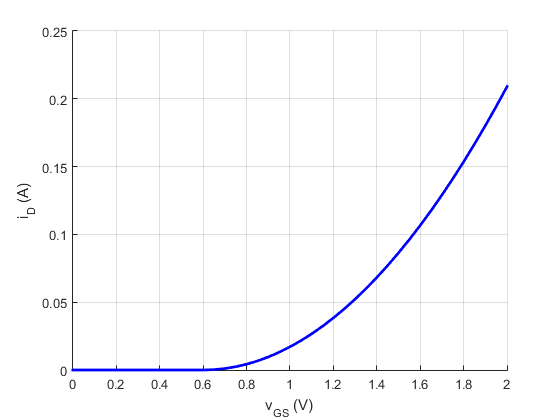
\includegraphics[width=.8\textwidth]{iD_vGS.png}
	\caption{Caractéristique de transfert}
\end{figure}

\begin{figure}[H]
	\centering
	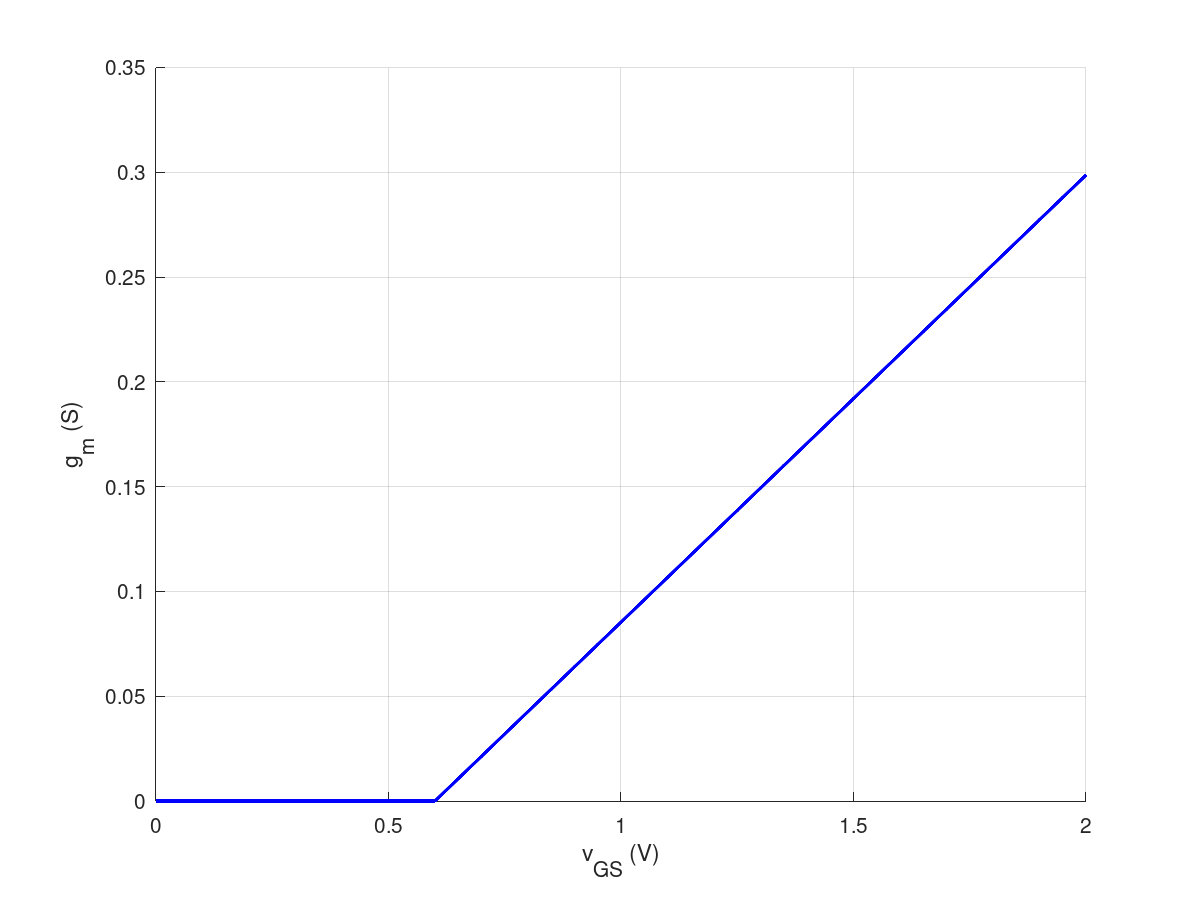
\includegraphics[width=.8\textwidth]{gm_vGS.png}
	\caption{Transconductance}
\end{figure}

\begin{figure}[H]
	\centering
	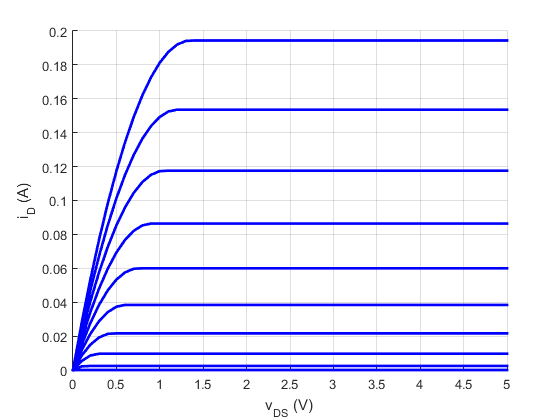
\includegraphics[width=.8\textwidth]{iD_vDS.png}
	\caption{Caractéristiques de sortie}
\end{figure}

\clearpage
\section{Caractéristiques du BS170}\label{an:bs170}
\centering
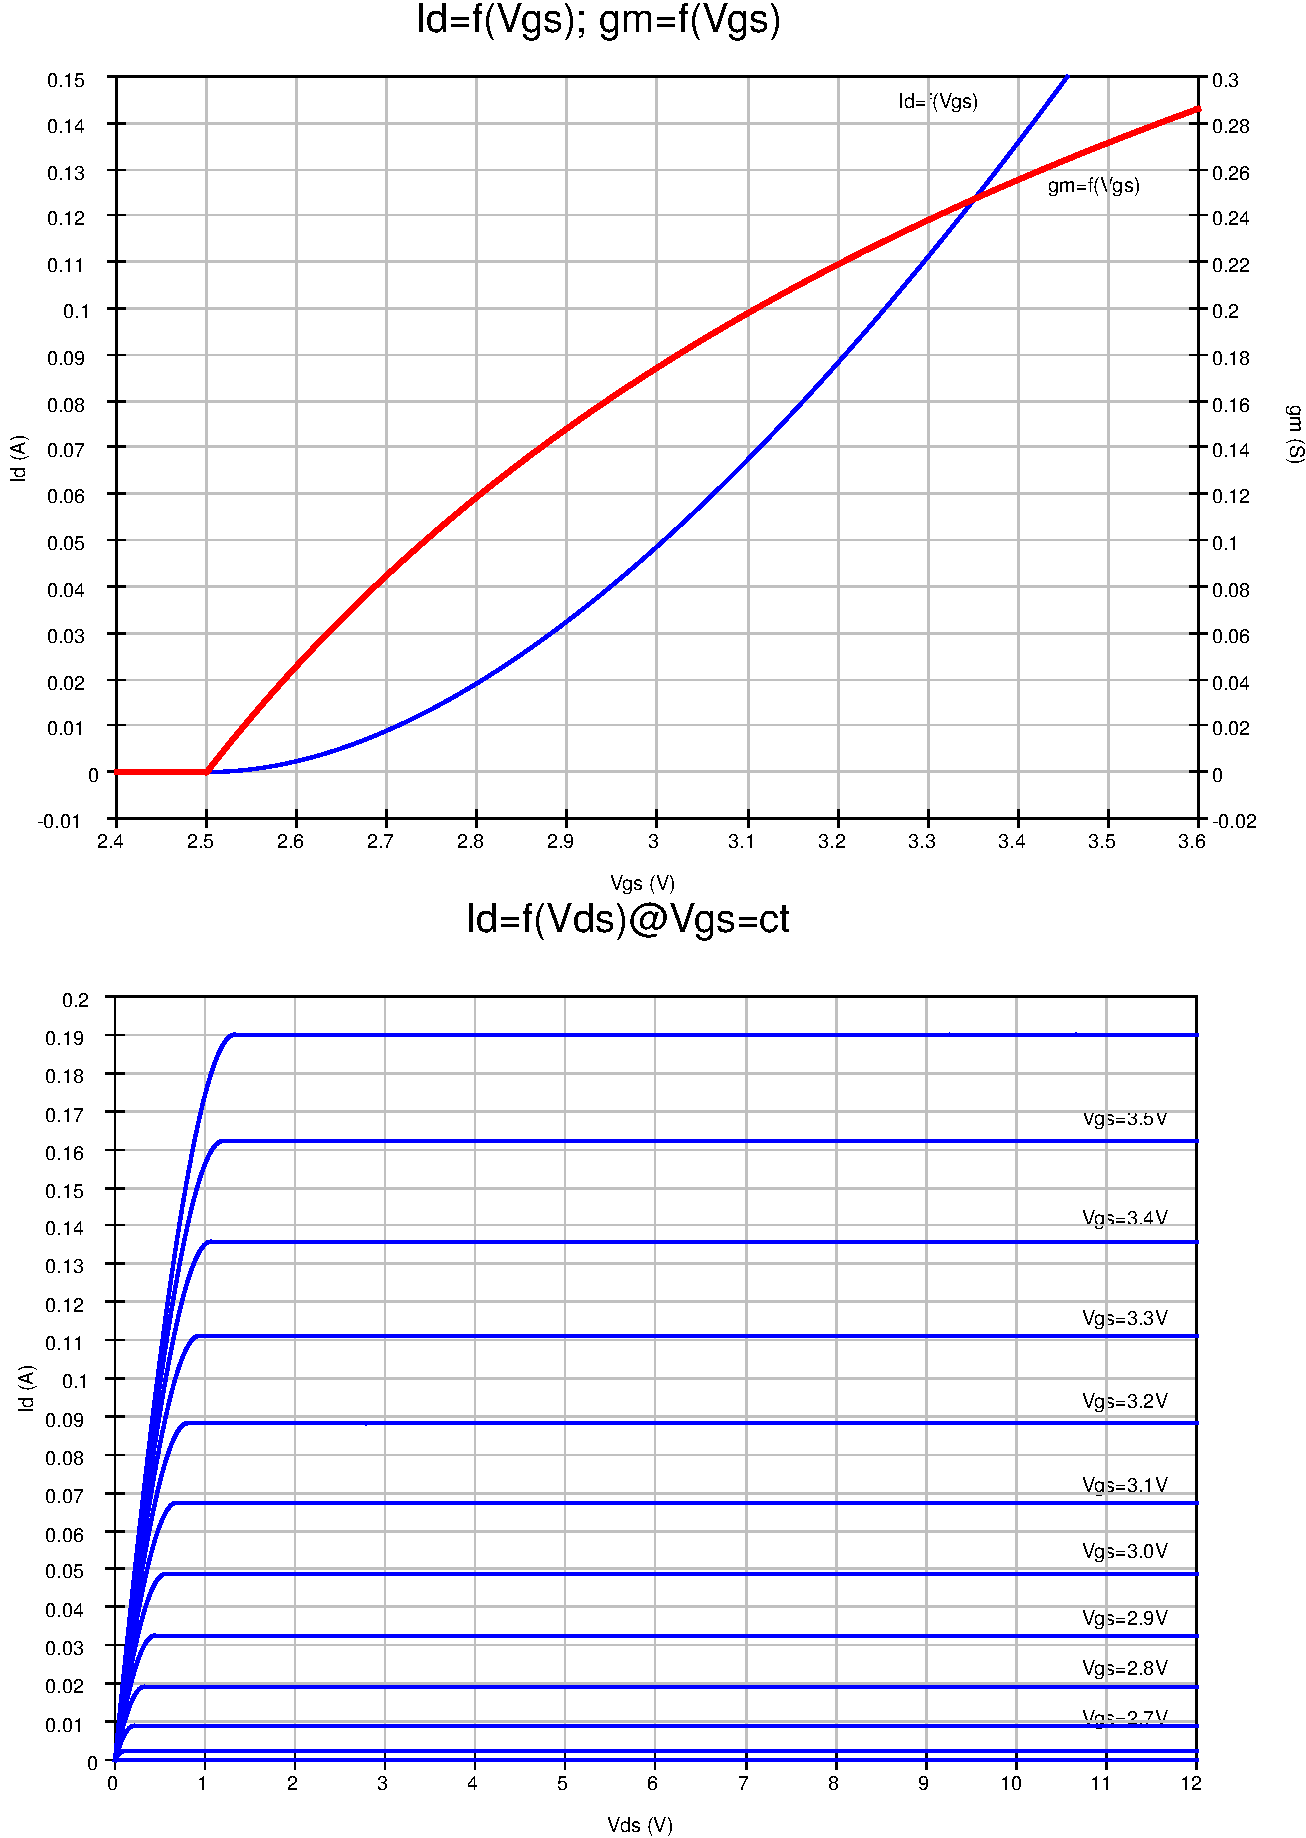
\includegraphics[width=\textwidth]{courbes_mos_2k16-crop.pdf}
%\newgeometry{top=1 in, bottom=1 in, left=1 in, right=1 in} % Yeah, that's bad to play with margins
% \section{Le transistor NMOS}
%
% \label{anx:mos}
% Le transistor NMOS est un transistor MOS à canal N.
%
% Le symbole utilisé est visible figure \vref{fig:mos_elec2}.
% \begin{figure}[H]
% 	\begin{center}
% 		\begin{circuitikz}[scale=0.8] \draw
% 		(2.25,1) node[nigfete] (mos) {}
% 		(mos.D) -- (2.25,2) to  [short, -o](3.25,2)  node[anchor=west] {D}
%
% 		(mos.S) -- (2.25,0) to [short, -o](3.25,0)  node[anchor=west] {S}
%
% 		(2.25,0) to [short, -o](0,0)  node[anchor=east] {S}
%
% 		(0,2)  node[anchor=east]{G}[short,o-] to  (1,2) -- (1,1) -- (mos.G)
% 		;\end{circuitikz}
% 	\end{center}\vspace{-0.7cm}
% \caption{Symbole du transistor NMOS}
% \label{fig:mos_elec2}
% \end{figure}
% \vspace{-1cm}

%
% \subsection{Régimes de fonctionnement}
% Le transistor MOS est utilisable selon 3 régimes de fonctionnement.
%
% Le changement de régime est conditionné principalement par la valeur de $V_{GS}$.
% \subsubsection{Coupure}
% Pour $V_{GS}<V_{TH}$, $I_D=0$
% \subsubsection{Zone Ohmique ou triode}
% Pour $V_{GS}>V_{TH}$ et $V_{GD}>V_{TH}$, le transistor fonctionne en zone ohmique :
% $$I_D=\mu _0 C_{ox} \frac{W}{L}\left( V_{GS} - V_{TH}- \frac{V_{DS}}{2}\right)V_{DS} $$
% avec les constantes :
% \begin{itemize}
% \item [$\mu _0$] mobilité des porteurs
% \item [$C_{ox}$] capacité surfacique de l'oxyde de grille
% \item [$W$] largeur du canal
% \item [$L$] longueur du canal
% \item [$V_{TH}$] tension de seuil
% \end{itemize}

% \subsubsection{Zone de Saturation}
% Pour $V_{GS}>V_{TH}$ et $V_{GD}<V_{TH}$, le transistor fonctionne en zone saturée :
% $$I_D=\mu _0 C_{ox} \frac{W}{2L}\left( V_{GS} - V_{TH} \right) ^2 $$
%
% Puisque $V_D$ est absent de cette équation, $V_D$ n'influence pas $I_D$ : dans cette zone, le transistor se comporte donc comme une source de courant constante -- dont la valeur $I_D$ dépend néanmoins de $V_{GS}$ (voir figure \ref{fig:ps}).
% La transconductance $g_m$ ($[S]$) est définie pour ce modèle par : $$g_m=\frac{\partial I_D}{\partial V_{GS}}$$
%
% \begin{figure}[H]
% 	\begin{center}
% 		\begin{circuitikz}[scale=0.8]\draw
% 			(0,0) node[anchor=east] {G}
% 			to [short, o-] (1,0)
% 			to [open, v=$V_{GS}$] (1,-2)
% 			to [short, -o] (0,-2)
% 			to  (0,-2) node[anchor=east] {S}
% 			to [short] (3,-2)
% 			(3,0) to [cI=$ g_m \cdot V_{GS}$] (3,-2)
% 			(3,-2) to [short, -o] (4,-2) node[anchor=west] {S}
% 			(3,0) to [short, -o] (4,0)
% 			to node[anchor=west] {D} (4,0)
% 		;\end{circuitikz}
% 	\end{center}\vspace{-1cm}
% \caption{Schéma équivalent du transistor en zone de saturation}
% \label{fig:ps}
% \end{figure}
% \vspace{-1.2cm}

% \section{Caractéristiques du transistor NMOS BS170}
% \label{anx:mos_doc}
% \begin{center}
% 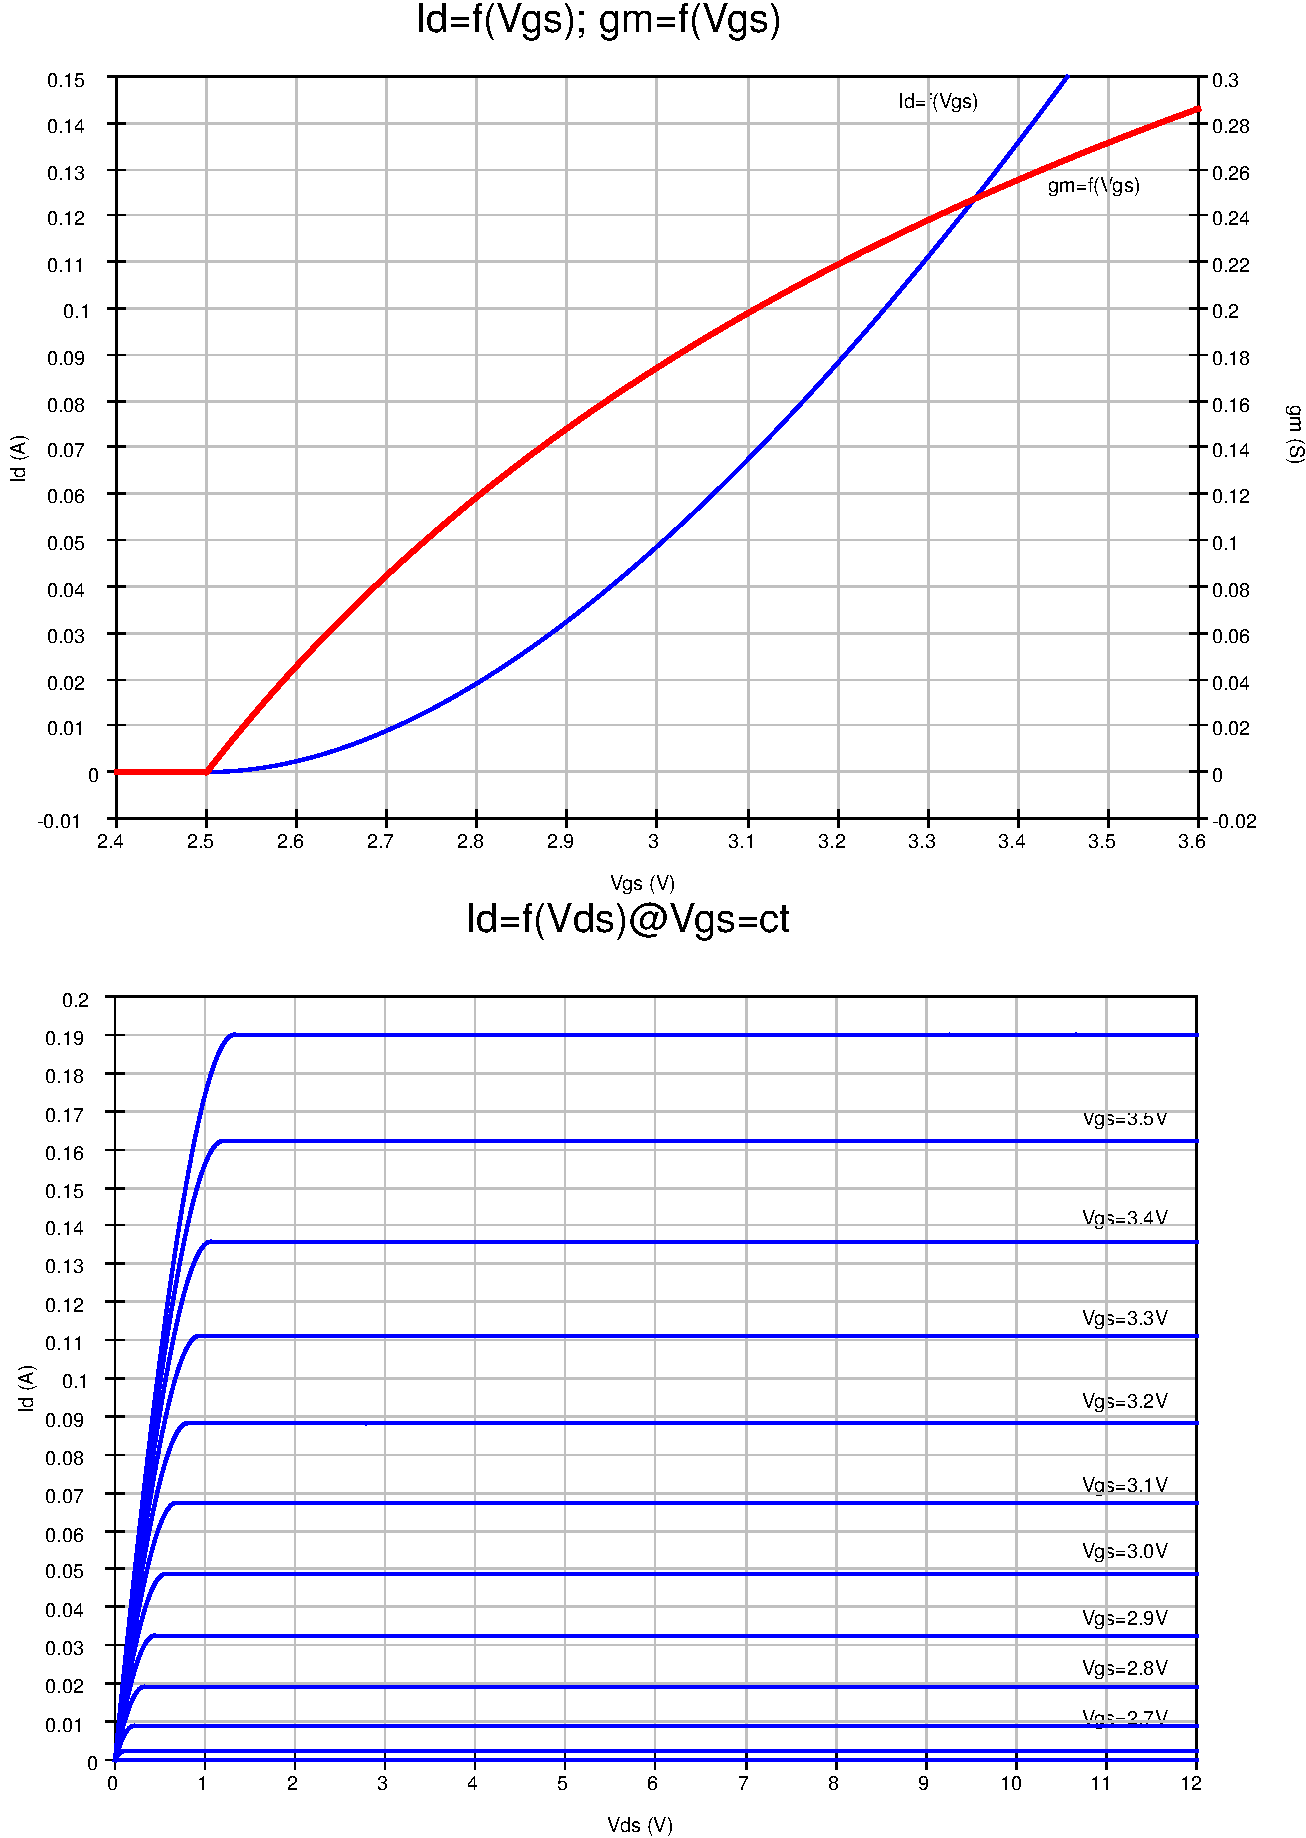
\includegraphics[width=16cm]{courbes_mos_2k16-crop.pdf}
% % les courbes ici sont ont été corrigée et sont cohérentes.
% \end{center}

% \phantomsection
% \addtocontents{toc}{
% \href{http://pdf.datasheetcatalog.com/datasheets/70/123316_DS.pdf}
% {\textbf{Documentation du transistor NMOS (lien cliquable)}}
% {\attachfile[icon=Graph, color=0 0.75 1,description =Documentation du transistor NMOS BS 170 ]{./Documentation_BS170.pdf}}}

% \label{anx:mos_datasheet}
%include pdf here
\end{document}
